\documentclass[9pt, ngerman]{beamer}
\usetheme[progressbar=frametitle]{metropolis}
\usecolortheme[snowy]{owl}

\usepackage{babel}
\usepackage{csquotes}
\usepackage{booktabs}
\usepackage{siunitx}
\usepackage{mhchem}
\usepackage{colortbl}


\usetikzlibrary{positioning}

\sisetup{
  locale = DE
}

\DeclareSIUnit
  \dH{{}^{\circ} dH}  % why the heck does SIUnitSymbolDegree not work?
\DeclareSIUnit[number-unit-product=\,]
  \dP{{}^{\circ} P}
\DeclareSIUnit[number-unit-product = {\%}]
  \volP{\,vol}
\DeclareSIUnit{\EUR}{EUR}

\newcommand{\forward}[1]{\textbf{→\,#1}}
\newcommand{\timelinesep}{\color{black!20}\makebox[0pt]{\tikz{\draw[fill=black!20] circle(0.3ex);}}\hskip-0.5pt\vrule width 1pt\hspace{\labelsep}}

\title{Der große Bierbrauworkshop}
\author{Arbeitskreis Kultur und Kommunikation --- Karlsruhe}
\date{24. September 2017}

\begin{document}
\maketitle

% http://www.cloneabeer.com/CABebc.php
\definecolor{ebc4}{RGB}{255, 230, 153}
\definecolor{ebc8}{RGB}{255, 191, 66}
\definecolor{ebc12}{RGB}{248, 166, 0}
\definecolor{ebc20}{RGB}{222, 124, 0}
\definecolor{ebc35}{RGB}{134, 24, 0}
\definecolor{ebc61}{RGB}{90, 10, 2}
\definecolor{ebc79}{RGB}{54, 8, 10}

\begin{frame}{Vorstellung}
  \begin{itemize}
    \item Max \& Matze brauen seit etwa fünf Jahren
    \item Wie ist euer Verhältnis zum Bier?
  \end{itemize}

  \begin{itemize}
    \item Mailingliste: \href{mailto:bier@lists.kit.edu}{bier@lists.kit.edu}
    \item Im Web: \href{http://noerdbier.de}{noerdbier.de}
    \item Auf GitHub: \href{https://gtihub.com/brewpeople}{github.com/brewpeople}
  \end{itemize}
\end{frame}

\section{Einführung}

\begin{frame}{Geschichtlicher Abriss}
  \begin{table}
    \renewcommand\arraystretch{1.4}\arrayrulecolor{red}
    \begin{tabular}{@{\,}r <{\hskip 2pt} !{\timelinesep}
      >{\raggedright\arraybackslash}p{8.5cm}}
      \addlinespace[1.5ex]
      10.000 v. Chr. & Erste archäologische Funde in Mesopotamien
        \begin{minipage}[t]{\linewidth}
          \begin{itemize}
            \item Bei Lagerung feucht gewordenes Getreide war süßer und
              nahrhafter
            \item Zu Brei verarbeitetes Getreide entwickelte nach einiger Zeit
              eine berauschende Wirkung
          \end{itemize}
        \end{minipage}\\
      3.000 v. Chr. & Erste Funde in Mitteleuropa\\
      2.000 v. Chr. & Erstes Braurezept in Keilschrift\\
      Mittelalter & Weiterentwicklung in Klöstern durch Zusatz von Eichenrinde und
        Kräutern\\
      14. Jhd. & Erste untergärige Biersorten, zunächst nur in kalten Regionen
        oder im Winter möglich
    \end{tabular}
  \end{table}
\end{frame}
\begin{frame}{Geschichtlicher Abriss}
  \begin{table}
    \renewcommand\arraystretch{1.4}\arrayrulecolor{red}
    \begin{tabular}{@{\,}r <{\hskip 2pt} !{\timelinesep}
      >{\raggedright\arraybackslash}p{8.5cm}}
      \addlinespace[1.5ex]
      16. Jhd. & Hopfen setzt sich als Konservierungsstoff durch\\
      1870 & Entwicklung der Kältemaschine durch \emph{Carl von Linde}
      ermöglicht flächendeckende Herstellung untergäriger Biere
    \end{tabular}
  \end{table}
\end{frame}
\begin{frame}{Reinheitsgebot}
  \begin{itemize}
    \item Marketingbegriff aus dem 20. Jahrhundert mit Bezug auf eine
      bayerische Vorschrift von 1516
    \item In den 50ern und 60ern in Auseinandersetzungen um Zuckerzusätze
      in nicht-bayerischen später nicht-deutschen Bieren benutzt
    \item \emph{Tag des Deutschen Bieres} am 23. April erinnert an Erlassung
      einer neuen bayerischen Landesordnung im Jahr 1516, in der es unter
      anderem heißt:

      \enquote{\emph{Wir wöllen auch sonnderlichen / das füran
      allenthalben in unsern Stetten / Märckthen / unnd auf dem Lannde / zu
      kainem Pier / merer Stuckh / dann \textbf{allain Gersten / Hopffen / und
      Wasser} /
      genomen unnd gepraucht sölle werden.}}
  \end{itemize}
\end{frame}
\begin{frame}{Definition}
  In Deutschland ist der Begriff und die Herstellung von \emph{Bier} durch die
  \emph{Verordnung zur Durchführung des Vorläufigen Biergesetzes} und das
  \emph{Vorläufige Biergesetz} von 1993 festgelegt.

  \begin{enumerate}
    \item[1.] Zur Bereitung von \textbf{untergärigem} Bier darf, abgesehen von den
      Vorschriften in den Absätzen 4 bis 6, nur \textbf{Gerstenmalz, Hopfen, Hefe und
      Wasser} verwendet werden.
    \item[2.] Die Bereitung von \textbf{obergärigem} Bier unterliegt derselben
      Vorschrift; es ist hierbei jedoch auch die Verwendung von \textbf{anderem
      Malz} und die Verwendung von technisch reinem Rohr-, Rüben- oder
      Invertzucker sowie von Stärkezucker und aus Zucker der bezeichneten Art
      hergestellten Farbmitteln zulässig.
  \end{enumerate}
\end{frame}
\begin{frame}{Definition}
  \begin{enumerate}
    \item[5.] An Stelle von Hopfen dürfen bei der Bierbereitung auch
      \textbf{Hopfenpulver} oder Hopfen in anderweit zerkleinerter Form oder
      Hopfenauszüge verwendet werden [\dots] Die Hopfenauszüge dürfen der
      Bierwürze nur \textbf{vor Beginn oder während der Dauer} des Würzekochens
      beigegeben werden.

    \item[6.] Als \textbf{Klärmittel} für Würze und Bier dürfen nur solche
      Stoffe verwendet werden, die mechanisch oder adsorbierend wirken und bis
      auf gesundheitlich, geruchlich und geschmacklich unbedenkliche, technisch
      unvermeidbare Anteile wieder ausgeschieden werden.
  \end{enumerate}
\end{frame}
\begin{frame}{Rechtliches}
  Bierbrauen ist nach dem \emph{Biersteuergesetz} grundsätzlich steuerpflichtig,
  wobei sich der Steuersatz nach \forward{Stammwürzegehalt} und Menge richtet
  (Stand 2017: \SI{0.787}{\EUR\per\dP\per\hL}) und bei Mengen unter
  \SI{200000}{\hL} stufenweise ermäßigt wird.

  Haus- und Hobbybrauer können bis zu \SI{2}{\hL} pro Kalenderjahr und Haushalt
  steuerfrei für den eigenen Verbrauch herstellen, müssen das dem Hauptzollamt
  aber formlos z.B. per Mail an
  \vspace{-0.5em}
  \begin{center}
    \href{mailto:poststelle.hza-karlsruhe@zoll.bund.de}{poststelle.hza-karlsruhe@zoll.bund.de}
  \end{center}
  \vspace{-0.5em}
  anzeigen. Für Demonstrationszwecke gilt dies leider nicht, weshalb wir heute
  für das Allgemeinwohl brauen.
\end{frame}

\section{Bierzutaten und -eigenschaften}

\begin{frame}{Zutaten}
  \begin{center}
    \vspace{2em}
    \begin{tikzpicture}[
        caption/.style={
          font=\bfseries,
        },
        cc-caption/.style={
          black!50,
          font=\tiny,
          anchor=north, yshift=2mm,
        },
    ]
      \node[] (malt) {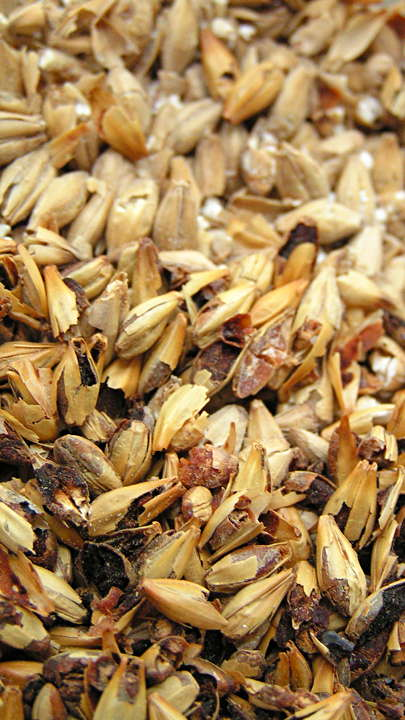
\includegraphics[width=2.5cm]{cc0/wikipedia-crystal-malt}};    % 405x720
      \node[right=1mm of malt]  (water) {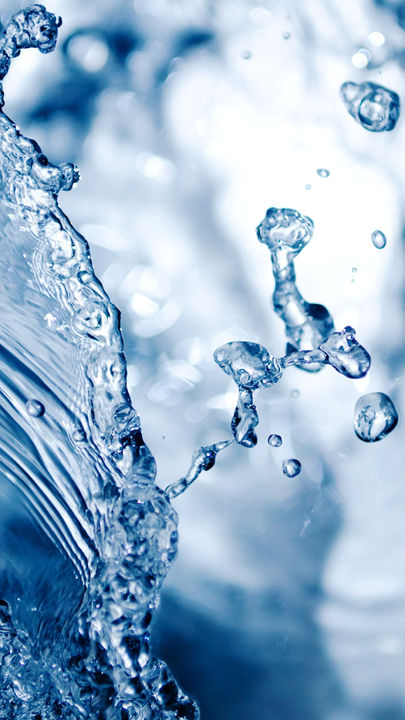
\includegraphics[width=2.5cm]{cc0/splashing-splash-aqua-water-pexels-photo-67843}};
      \node[right=1mm of water] (hops)  {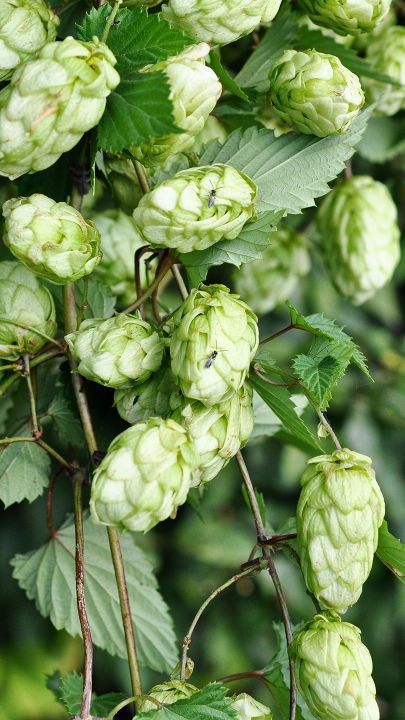
\includegraphics[width=2.5cm]{cc-sa/wikipedia-hops.jpg}};
      \node[right=1mm of hops]  (yeast) {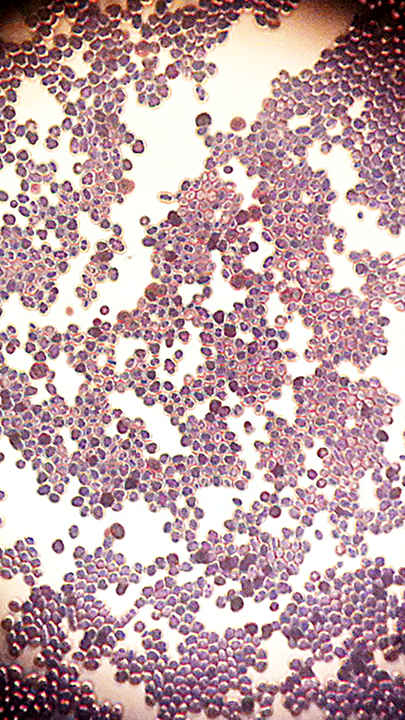
\includegraphics[width=2.5cm]{cc-sa/wikipedia-saccharomyces-cerevisiae.jpg}};

      \node[below=1mm of malt, caption]   {Getreidemalze\strut};
      \node[below=1mm of water, caption]  {Wasser\strut};
      \node[below=1mm of hops, caption]   {Hopfen\strut};
      \node[below=1mm of yeast, caption]  {Hefe\strut};

      \node[cc-caption] (hops-attr) at (hops.south)     {CC-BY-SA 4.0/Lazaregagnidze};
      \node[cc-caption] (yeast-attr) at (yeast.south)   {CC-BY-SA 4.0/A doubt};
    \end{tikzpicture}
  \end{center}
\end{frame}
\begin{frame}{Malz}

  Aus Getreiden wie \emph{Gerste} und \emph{Weizen} -- seltener auch
  \emph{Roggen} und \emph{Dinkel} -- entstehen beim Mälzen durch
  Einweichen und Keimung verschiedene Enzyme, insbesondere \forward{Amylasen}
  zur Umwandlung von Stärke in Zucker.

  Nach wenigen Tagen wird die Keimung durch Trocknung (Darren) unterbrochen und
  der Keimling entfernt.

  Zur besseren \forward{Läuterung} wird das Malz geschrotet und nicht gemahlen.
\end{frame}
\begin{frame}{Bierfarbe}
  \tikzset{
    ebc bar/.style={
      rectangle,
      minimum width=2cm,
    }
  }

  Die Bierfarbe hängt maßgeblich von der Farbe des Malzes ab, die durch
  Temperatur beim Darren festgelegt wird. Der von der \textbf{E}uropean
  \textbf{B}rewery \textbf{C}onvention festgelegte EBC-Wert beschreibt wie viel
  Licht absorbiert wird und entspricht grob einem Farbgradienten von hellgelb zu
  tiefbraun:

  \begin{table}
    \begin{tabular}{llll}
      \textbf{EBC} & \textbf{englisch} & \textbf{deutsch} & \textbf{Farbe}\\
      \midrule
      4--8  & pale & hell & \tikz {\node[ebc bar, left color=ebc4, right color=ebc8] {}} \\
      8--12 & golden, pale & gold & \tikz {\node[ebc bar, left color=ebc8, right color=ebc12] {}} \\
      12--20 & amber & bernstein & \tikz {\node[ebc bar, left color=ebc12, right color=ebc20] {}} \\
      20--35 & light brown, copper & kupfer & \tikz {\node[ebc bar, left color=ebc20, right color=ebc35] {}} \\
      35--60 & brown & braun & \tikz {\node[ebc bar, left color=ebc35, right color=ebc61] {}} \\
      60+ & dark brown, black & schwarz & \tikz {\node[ebc bar, left color=ebc61, right color=ebc79] {}}
    \end{tabular}
  \end{table}
\end{frame}
\begin{frame}{Wasser}

  Wasser ist der Hauptbestandteil der \forward{Maische} als auch des endgültigen
  Bierprodukts. Die Wasserhärte und der pH-Wert bestimmen, welche Malze genutzt
  und schlussendlich welche Biere gebraut werden können.

  Enzyme die in der Maische Stärke in Zucker umsetzen, arbeiten optimal bei
  leicht saurem Millieu und einem pH-Wert von \numrange{5.5}{6.5}.
  Das Malz enthält von Natur aus bereits Stoffe, welche den pH-Wert senken.
  Je dunkler das Malz desto stärker senkt dieses den pH-Wert.

  Die Härte des Wassers hat ebenfalls Einfluss auf den Brauprozess da ein Teil der für
  die Härte verantwortlichen Ionen den pH-Wert beeinflussen und die Säure aus dem Malz neutralisieren.
  Die \emph{Restalkalität} ist ein Maß für die säurevernichtenden Anionen im Wasser.

  % Sehr umfangreiche Informationen zum Thema Wasser bietet:

  % \url{http://braumagazin.de/article/von-der-wasseranalyse-zum-brauwasser}
\end{frame}
\begin{frame}{Wasser und Bierstile}
  \begin{block}{Karlsruher Wasser}
    \vspace{0.5em}
    pH-Wert von \num{7.1} ist gut genug, allerdings ist das Wasser mit einer
    Rest\-al\-ka\-li\-tät von etwa \SI{10}{\dH} sehr hart, womit ohne Wasserbehandlung
    nur \textbf{Weizen-} und \textbf{dunkle Biere} ihr volles Aroma entwickeln
    können.
  \end{block}

  \sisetup{range-phrase = --}
  \begin{table}
    \begin{tabular}{lrrr}
      \textbf{Bierstil} & \textbf{Restalkalität \si{\dH}} & \textbf{Calcium \si{\milli\gram\per\liter}} & \textbf{Magnesium \si{\milli\gram\per\liter}}\\
      \midrule
      Helles    & \numrange{-3}{0} & \numrange{30}{50}  & \numrange{0}{20} \\
      Pils      & \numrange{-5}{0} & \numrange{0}{75}   & \numrange{0}{20} \\
      Bock      & \numrange{5}{10} & \numrange{50}{75}  & \numrange{0}{20} \\
      Weizen    & \numrange{5}{10} & \numrange{50}{100} & \numrange{0}{20}
    \end{tabular}
  \end{table}
\end{frame}
\begin{frame}{Hopfen}

  Hopfen fördert die \emph{Haltbarkeit} und ist verantwortlich für den
  herb-bitteren Geschmack eines Bieres. Verschiedene Hopfen werden als
  \emph{Bitterhopfen} zu Beginn oder als \emph{Aromahopfen} am Ende des
  \forward{Hopfenkochens} zugegeben.

  \begin{columns}[onlytextwidth]
    \begin{column}{0.6\textwidth}

      Die International Bitterness Unit (IBU) ist die Maßeinheit für den
      α-Säure-Anteil im Bier.

      Im Allgemeinen steigt der Bittereindruck mit höherer IBU, sinkt allerdings
      bei höherem Malzanteil weshalb schwere Biere höheren IBU für denselben
      Bittereindruck benötigen.

    \end{column}

    \begin{column}{0.4\textwidth}
      \sisetup{range-phrase = --}
      \begin{table}
        \begin{tabular}{ll}
          \textbf{IBU} & \textbf{Bierstil}\\
          \midrule
          \numrange{0}{8}   & Berliner Weisse\\
          \numrange{18}{25} & Kölsch\\
          \numrange{20}{40} & Porter\\
          \numrange{30}{45} & Pils\\
          40+               & India Pale Ale\\
        \end{tabular}
      \end{table}
    \end{column}
  \end{columns}

\end{frame}
\begin{frame}{Stammwürze}

  Der Stammwürzegehalt ist der Anteil der aus Malz und Hopfen im Wasser gelösten
  Stoffe (Extrakt), wird in Grad Plato (\si{\dP})  angegeben und entspricht der
  Massendichte einer wässrigen Saccharoselösung mit einem Gewichtsprozent
  Saccharose.

  \begin{block}{Messung}
    \vspace{0.5em}
    Der Wert wird über die Bierspindel oder einem Refraktometer ermittelt.
    Hierbei ist auf die korrekte Kalibrierung insbesondere im Hinblick auf die
    Temperatur der Würze zu achten.
  \end{block}
\end{frame}
\begin{frame}{Hefe}

  Die Hefe führt zur \forward{Vergärung} des Zuckers zu Kohlenstoffdioxid und
  Ethanol.

  Alle Hefesorten lassen sich grob in \emph{untergärige} und \emph{obergärige}
  Hefen einteilen. Untergärige Hefen benötigen Gärtemperaturen zwischen
  \SIrange{4}{9}{\celsius}, während obergärige Hefen bereits bei
  Zimmertemperatur (\SIrange{15}{22}{\celsius}) zur Gärung führen.

\end{frame}

\section{Biertypen}

\begin{frame}{Einteilung}
  % \begin{block}{Gattung, Sorte und Typ}

  Die \emph{Biergattung} ergibt sich aus dem \forward{Stammwürzegehalt} vor der
  \forward{Gärung}. Verkehrsübliche Bezeichnungen (z.B. Lagerbier, Exportbier)
  werden zu \emph{Biersorten} zusammengefasst währen der \emph{Biertyp} durch lokale
  Gegebenheiten charakterisiert wird.

  \begin{table}
    \begin{tabular}{lrll}
      \textbf{Gattung} & \textbf{Stammwürze} & \textbf{obergärig} & \textbf{untergärig}\\
      \midrule
      Einfachbier & \SIrange{2}{6}{\percent}    & Süßbier & \\
      Schankbier  & \SIrange{7}{10}{\percent}    & Berliner Weiße & \\
      Vollbier    & \SIrange{11}{15}{\percent}  & Alt, Kölsch, Weizen & Pils, Lager, Export \\
      Starkbier   & ab \SI{16}{\percent}         & Weizenbock & Bock \\
    \end{tabular}
  \end{table}
\end{frame}
\begin{frame}{Untergärige Biertypen}
  \begin{table}
    \begin{tabular}{llllll}
      \textbf{Kategorie} & \textbf{StW \textdegree P} & \textbf{IBU} & \textbf{EBC} & \textbf{\% vol} \\
      \midrule
      Leichtes Lager & 7,0--13,8 & 8--30 & 4--12 & 2,8--6,0 \\
      Pils & 11,0--14,7 & 25--45 & 4--12 & 4,4--6,0 \\
      Europ. bernsteinf. Lager & 11,4--14,0 & 18--30 & 14--32 & 2,6--5,7 \\
      Dunkles Lager & 11,0--13,8 & 8--32 & 28--59 & 4,2--6,0 \\
      Bock & 15,7--28,0 & 16--35 & 12--59 & 6,3--14,0 \\
    \end{tabular}
  \end{table}
\end{frame}
\begin{frame}{Obergärige Biertypen -- Ales}
  \begin{table}
    \begin{tabular}{llllll}
      \textbf{Kategorie} & \textbf{StW \textdegree P} & \textbf{IBU} & \textbf{EBC} & \textbf{\% vol} \\
      \midrule
      English Pale Ale & 8,0--14,7 & 23--50 & 8--35 & 3,2--6,2 \\
      Scot./Irish Pale Ale & 7,6--30,1 & 10--35 & 18--49 & 2,5--10,0 \\
      American Ale & 11,2--14,7 & 20--45 & 10--69 & 4,3--6,2 \\
      English Brown Ale & 7,6--12,9 & 10--30 & 24--69 & 2,8--5,4 \\
      India Pale Ale & 12,4--21,6 & 40--120 & 12--30 & 5,0--10,0 \\
      Belg./Franz. Ale & 11,0--19,3 & 10--35 & 4--37 & 4,5--8,5 \\
      Belg. Starkbier & 15,2--25,9 & 15--40 & 6--43 & 6,0--11,0 \\
      Strong Ale & 14,7--28,0 & 30--120 & 16--43 & 6,0--12,0
    \end{tabular}
  \end{table}
\end{frame}
\begin{frame}{Obergärige Biertypen -- andere}
  \begin{table}
    \begin{tabular}{llllll}
      \textbf{Kategorie} & \textbf{StW \textdegree P} & \textbf{IBU} & \textbf{EBC} & \textbf{\% vol} \\
      \midrule
      Helles Hybrid & 9,5--13,6 & 15--30 & 5--12 & 2,1--5,6 \\
      Bernsteinf. Hybrid & 11,4--13,3 & 25--50 & 20--33 & 4,5--5,5 \\
      Porter & 10,0--21,6 & 18--50 & 33--69 & 4,5--9,5 \\
      Stout & 9,0--27,0 & 25--90 & 43--79 & 4,0--12,0 \\
      Weizen- u. Roggenbier & 11,0--21,6 & 8--30 & 4--49 & 4,3--8,0 \\
      Sauerbier & 7,1--18,0 & 0--25 & 4--43 & 2,8--8,0
    \end{tabular}
  \end{table}
\end{frame}

\section{Der Brauprozess}

\begin{frame}{Überblick}
  \begin{center}
    \vspace{0.5cm}
    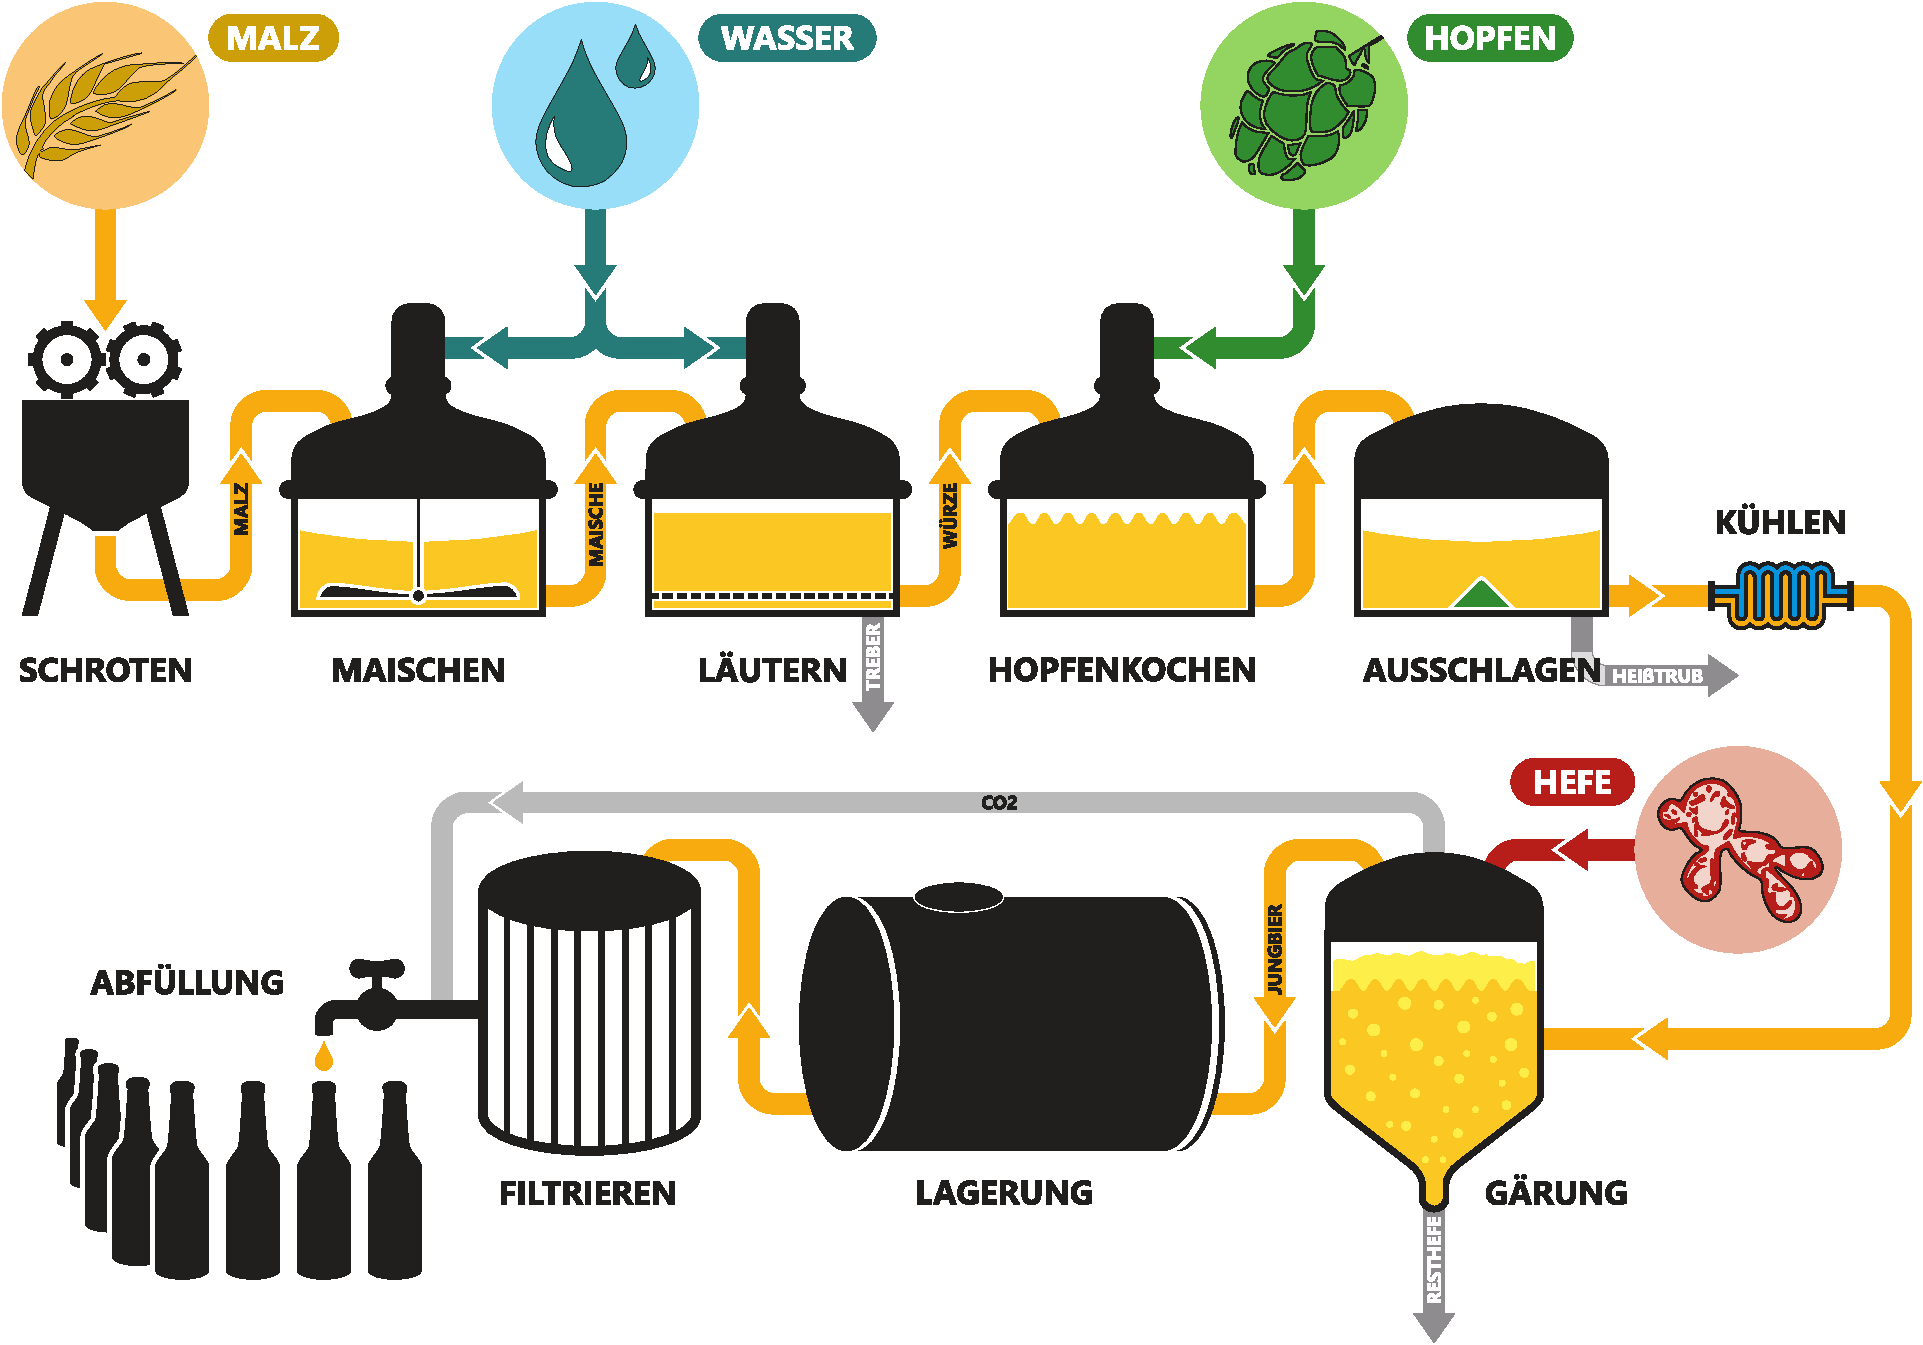
\includegraphics[width=\textwidth]{pdfs/prozess-ueberblick.pdf}
  \end{center}
\end{frame}
\begin{frame}{Maischen}
  \begin{center}
    \vspace{0.5cm}
    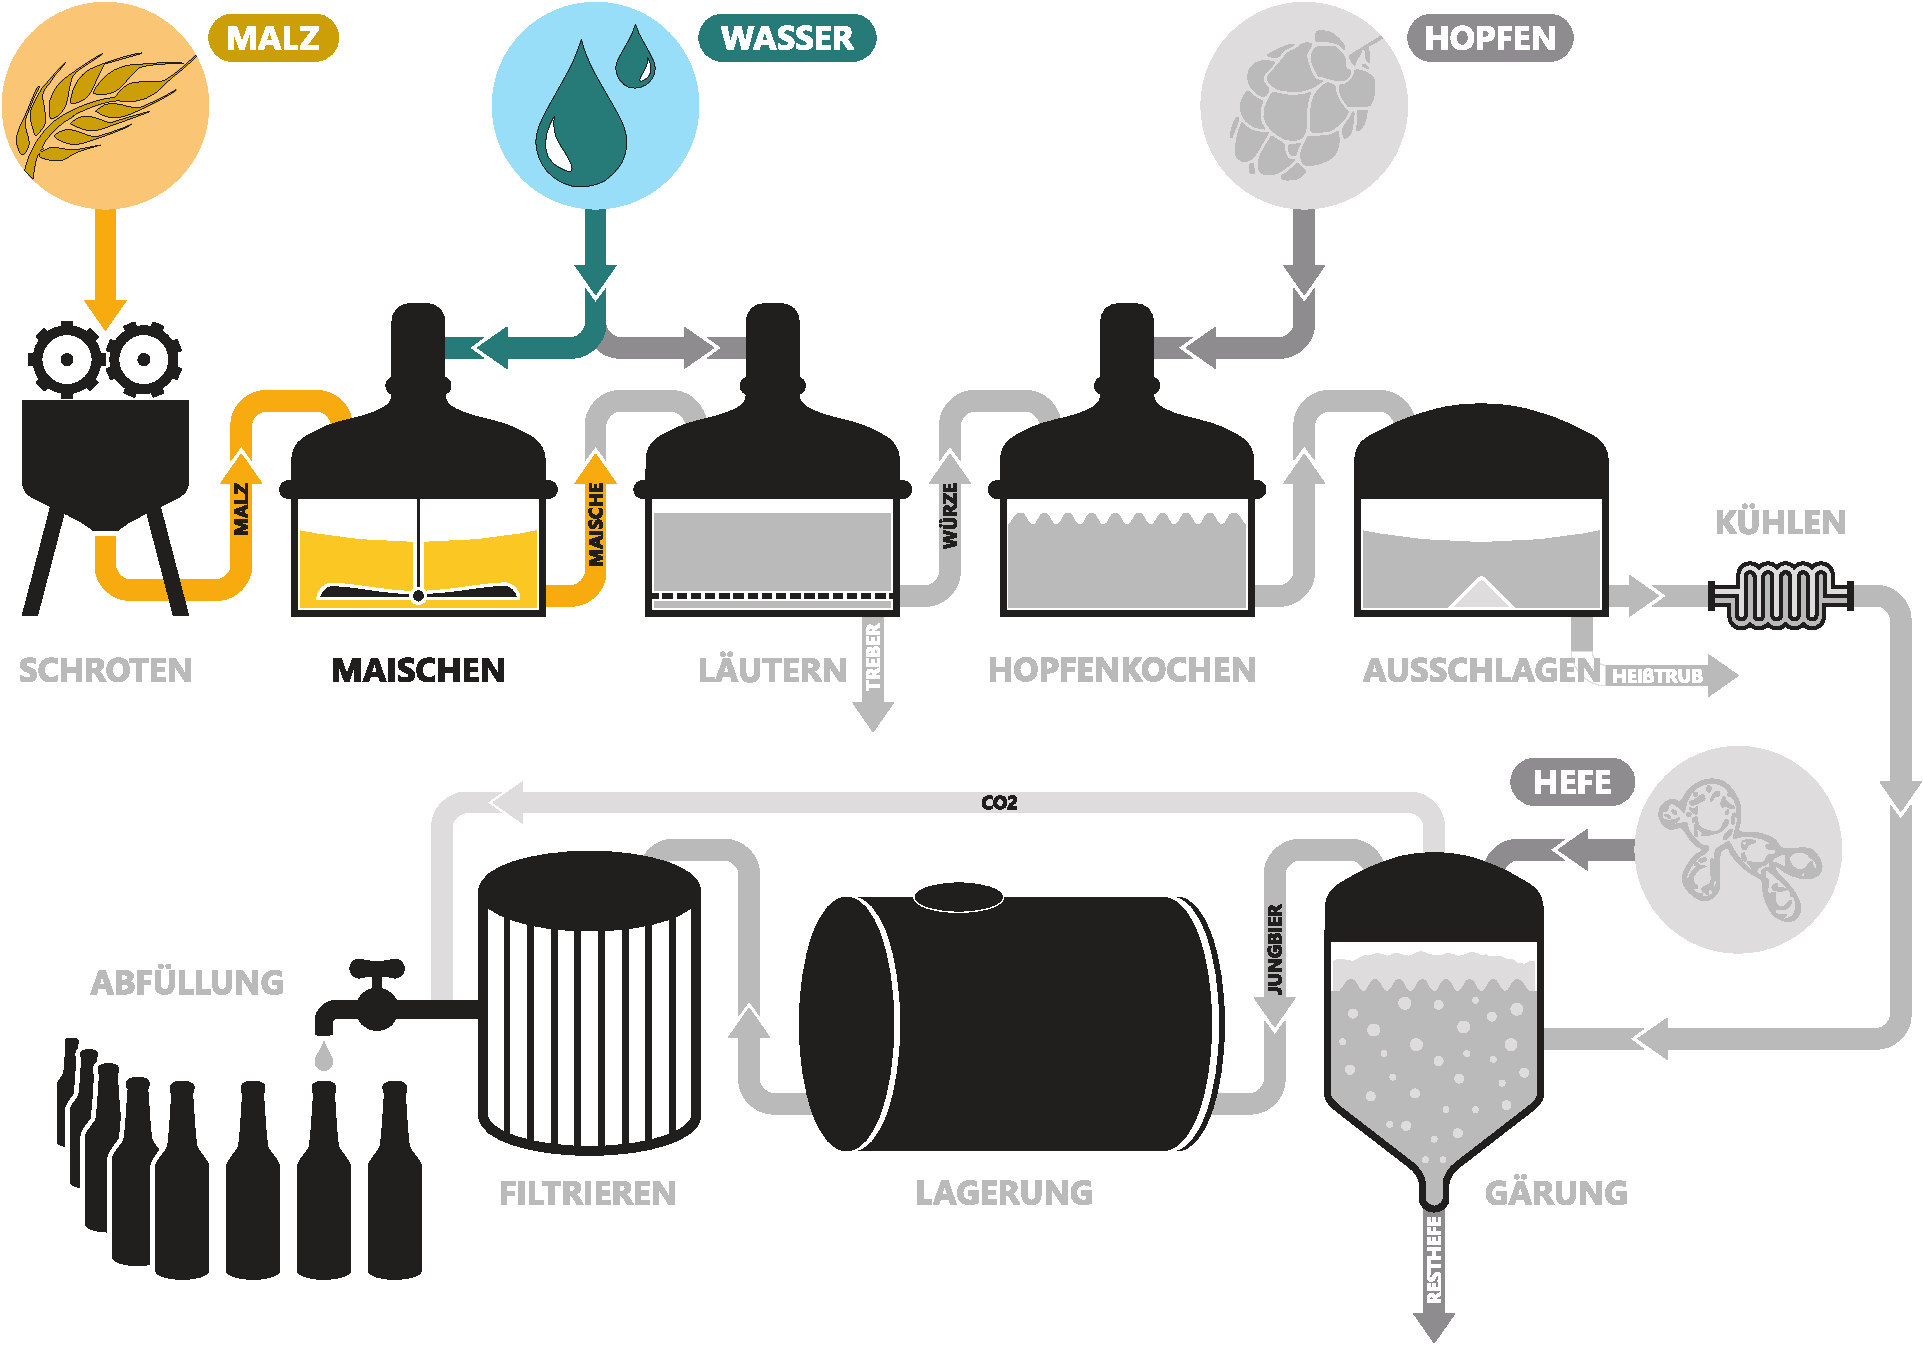
\includegraphics[width=\textwidth]{pdfs/prozess-maischen.pdf}
  \end{center}
\end{frame}
\begin{frame}{Maischen}
  \begin{block}{Zweck}
    \vspace{0.5em}

    Abbau der Stärke im Malz durch Enzyme wie β-Amylase zu
    \emph{vergärbarer Maltose} und α-Amylase zu \emph{unvergärbaren
    Dextrinen}.

  \end{block}

  \begin{block}{Maischeverfahren}
  	\begin{description}
  		\item[Deduktion] Teil der Maische wird entnommen, separat gekocht und wieder zugegeben
  		\item[Infusion] Stufenweise Zugabe kochenden Wassers
  		\item[Kesselmaische] Gesamte Maische wird in Kessel stufenweise aufgeheizt
  	\end{description}
  \end{block}
\end{frame}
\begin{frame}{Maischen}
  \begin{block}{Typischer Ablauf Kesselmaische}
    \begin{enumerate}
      \item Zugabe der Schüttung zum Wasser bei \emph{Einmaischtemperatur}
      \item \emph{Maltoserast} bei etwa \SI{63}{\degree\celsius}, Zerstörung der
        β-Amylase ab \SI{65}{\degree\celsius}
      \item \emph{Verzuckerungsrast} bei etwa \SI{73}{\degree\celsius},
        Zerstörung der α-Amylase ab \SI{80}{\degree\celsius}
    \end{enumerate}
  \end{block}
  \begin{block}{Weitere Rasten}
    \vspace{-0.5em}
    \begin{table}
      \sisetup{range-phrase = --}
      \begin{tabular}{lrrrr}
        \textbf{Name} & \textbf{Bereich \si{\degree\celsius}} & \textbf{Optimal \si{\degree\celsius}} & \textbf{Dauer \si{\minute}}\\
        \midrule
        Gummirast           & \numrange{35}{40} & 39        & \numrange{15}{30}\\
        Weizenrasten        & ---               & 45 \& 48  & je ca. 15\\
        Eiweißrast          & \numrange{50}{58} & 52        & \numrange{10}{20}\\
        Maltoserast         & \numrange{60}{68} & 63        & \numrange{30}{90}\\
        Verzuckerungsrast   & \numrange{68}{76} & 72        & \numrange{15}{30}\\
        Abmaischen          & \numrange{77}{80} & 78        & min. 20\\
      \end{tabular}
    \end{table}
  \end{block}
\end{frame}
\begin{frame}{Läutern}
  \begin{center}
    \vspace{0.5cm}
    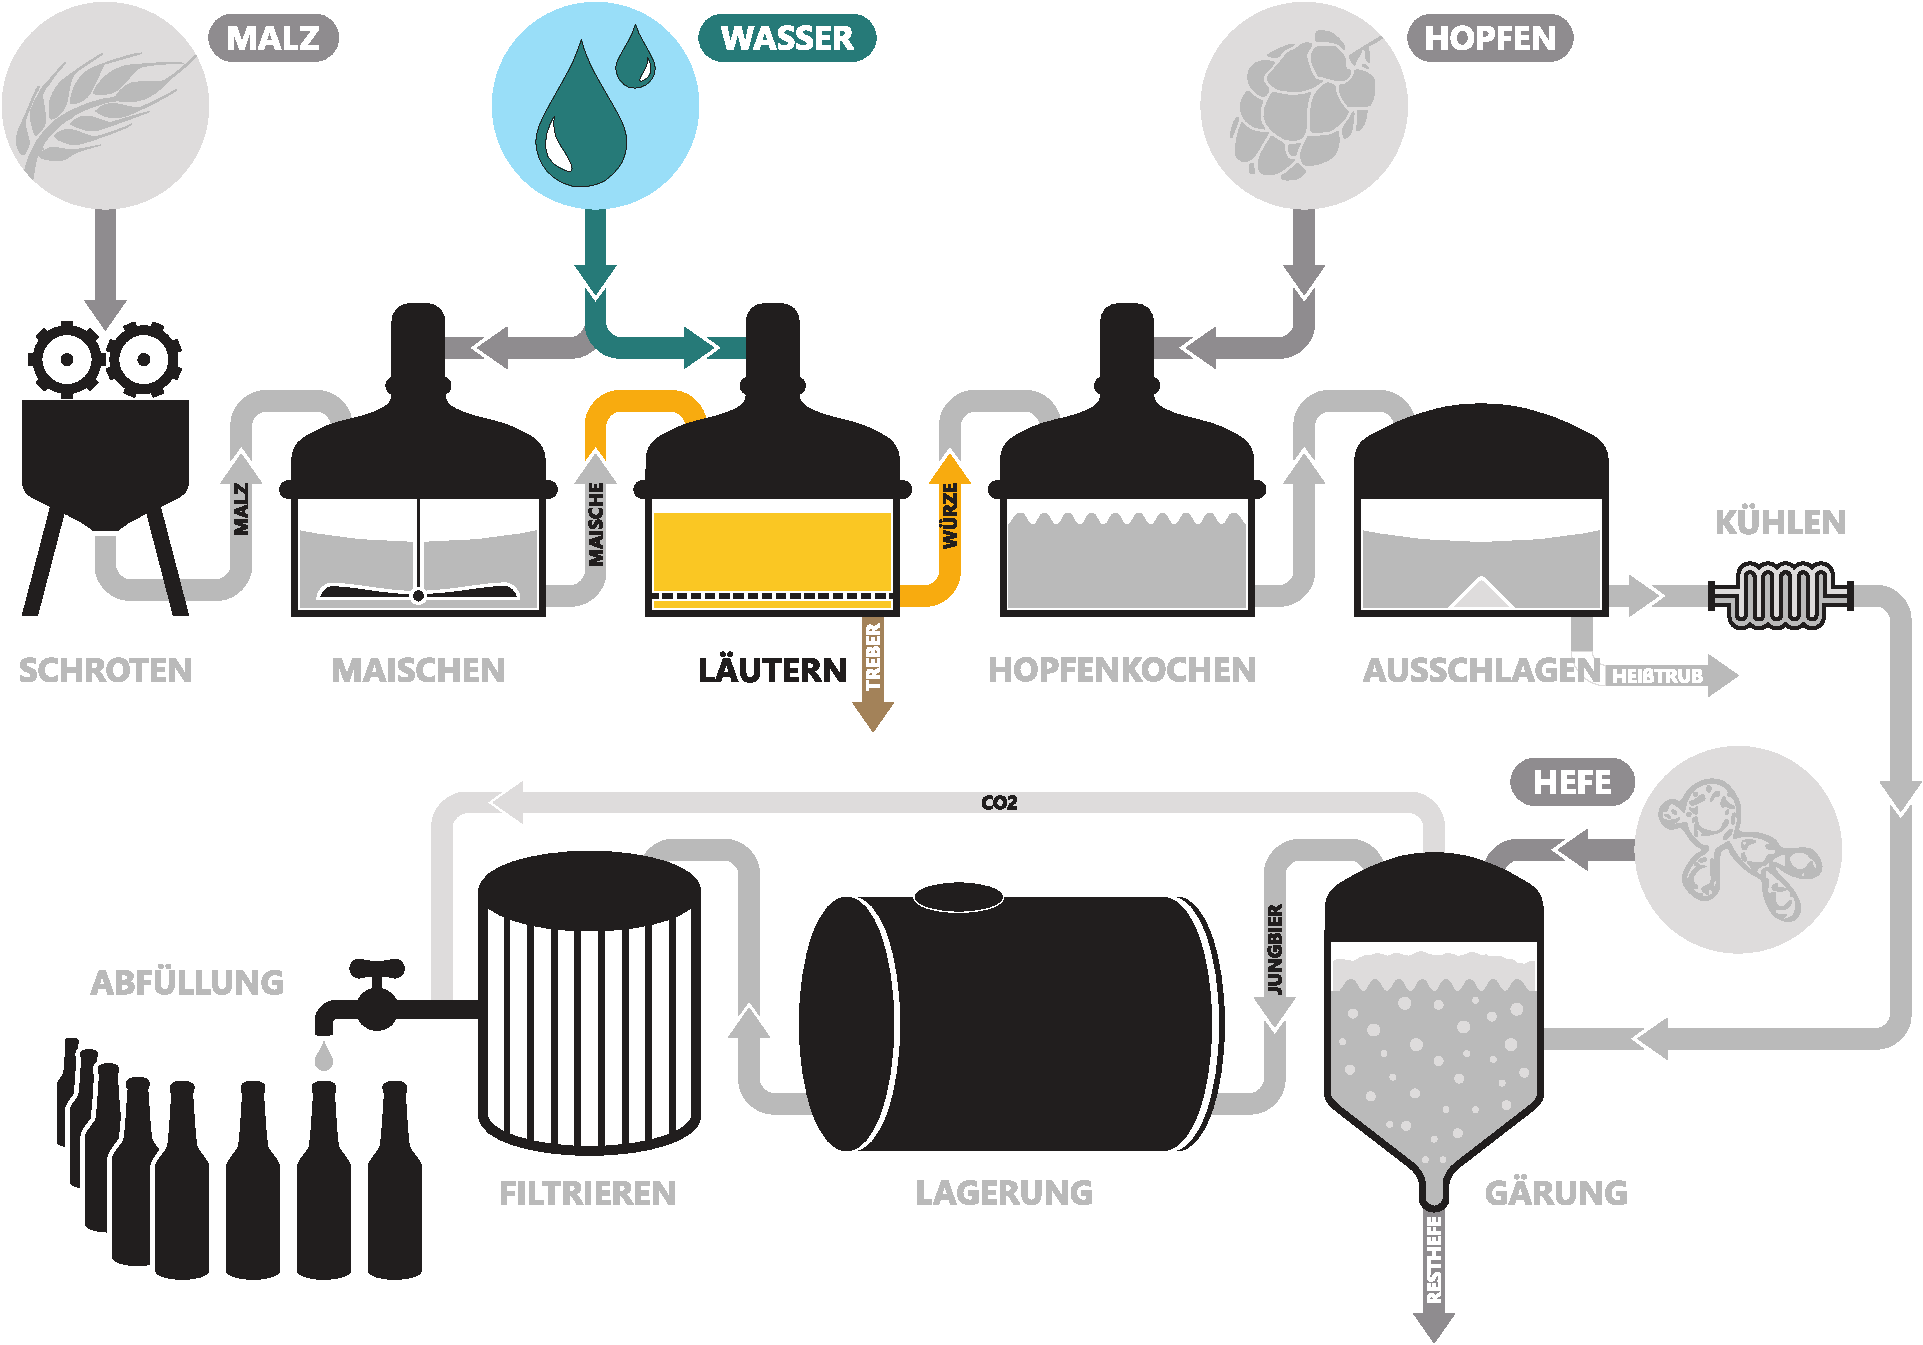
\includegraphics[width=\textwidth]{pdfs/prozess-laeutern.pdf}
  \end{center}
\end{frame}
\begin{frame}{Läutern}
  \begin{block}{Zweck}
    \vspace{0.5em}

    Trennung der wässrigen Lösung (\emph{Würze}) von den ungelösten Feststoffen
    (\emph{Treber}), wozu die Filtrationseigenschaft des Trebers im
    \emph{Hauptguss} genutzt wird. Zur optimalen Ausbeute werden im
    \emph{Nachguss} Restzucker aus dem Treber gelöst.

  \end{block}

  \begin{block}{Ablauf}
    \begin{enumerate}
      \item Umfüllung der Maische in den \emph{Läuterbottich}
      \item \emph{Läuterruhe} zum Absetzen des Trebers
      \item Rückführung der Würze in den Läuterbottich bis sie aufklart
      \item Ableiten der klaren Würze in den Braukessel
      \item \emph{Anschwänzen} des Trebers mit \SIrange{75}{80}{\degree\celsius}
        vorgewärmtem Nachguss
    \end{enumerate}
  \end{block}
\end{frame}
\begin{frame}{Hopfenkochen}
  \begin{center}
    \vspace{0.5cm}
    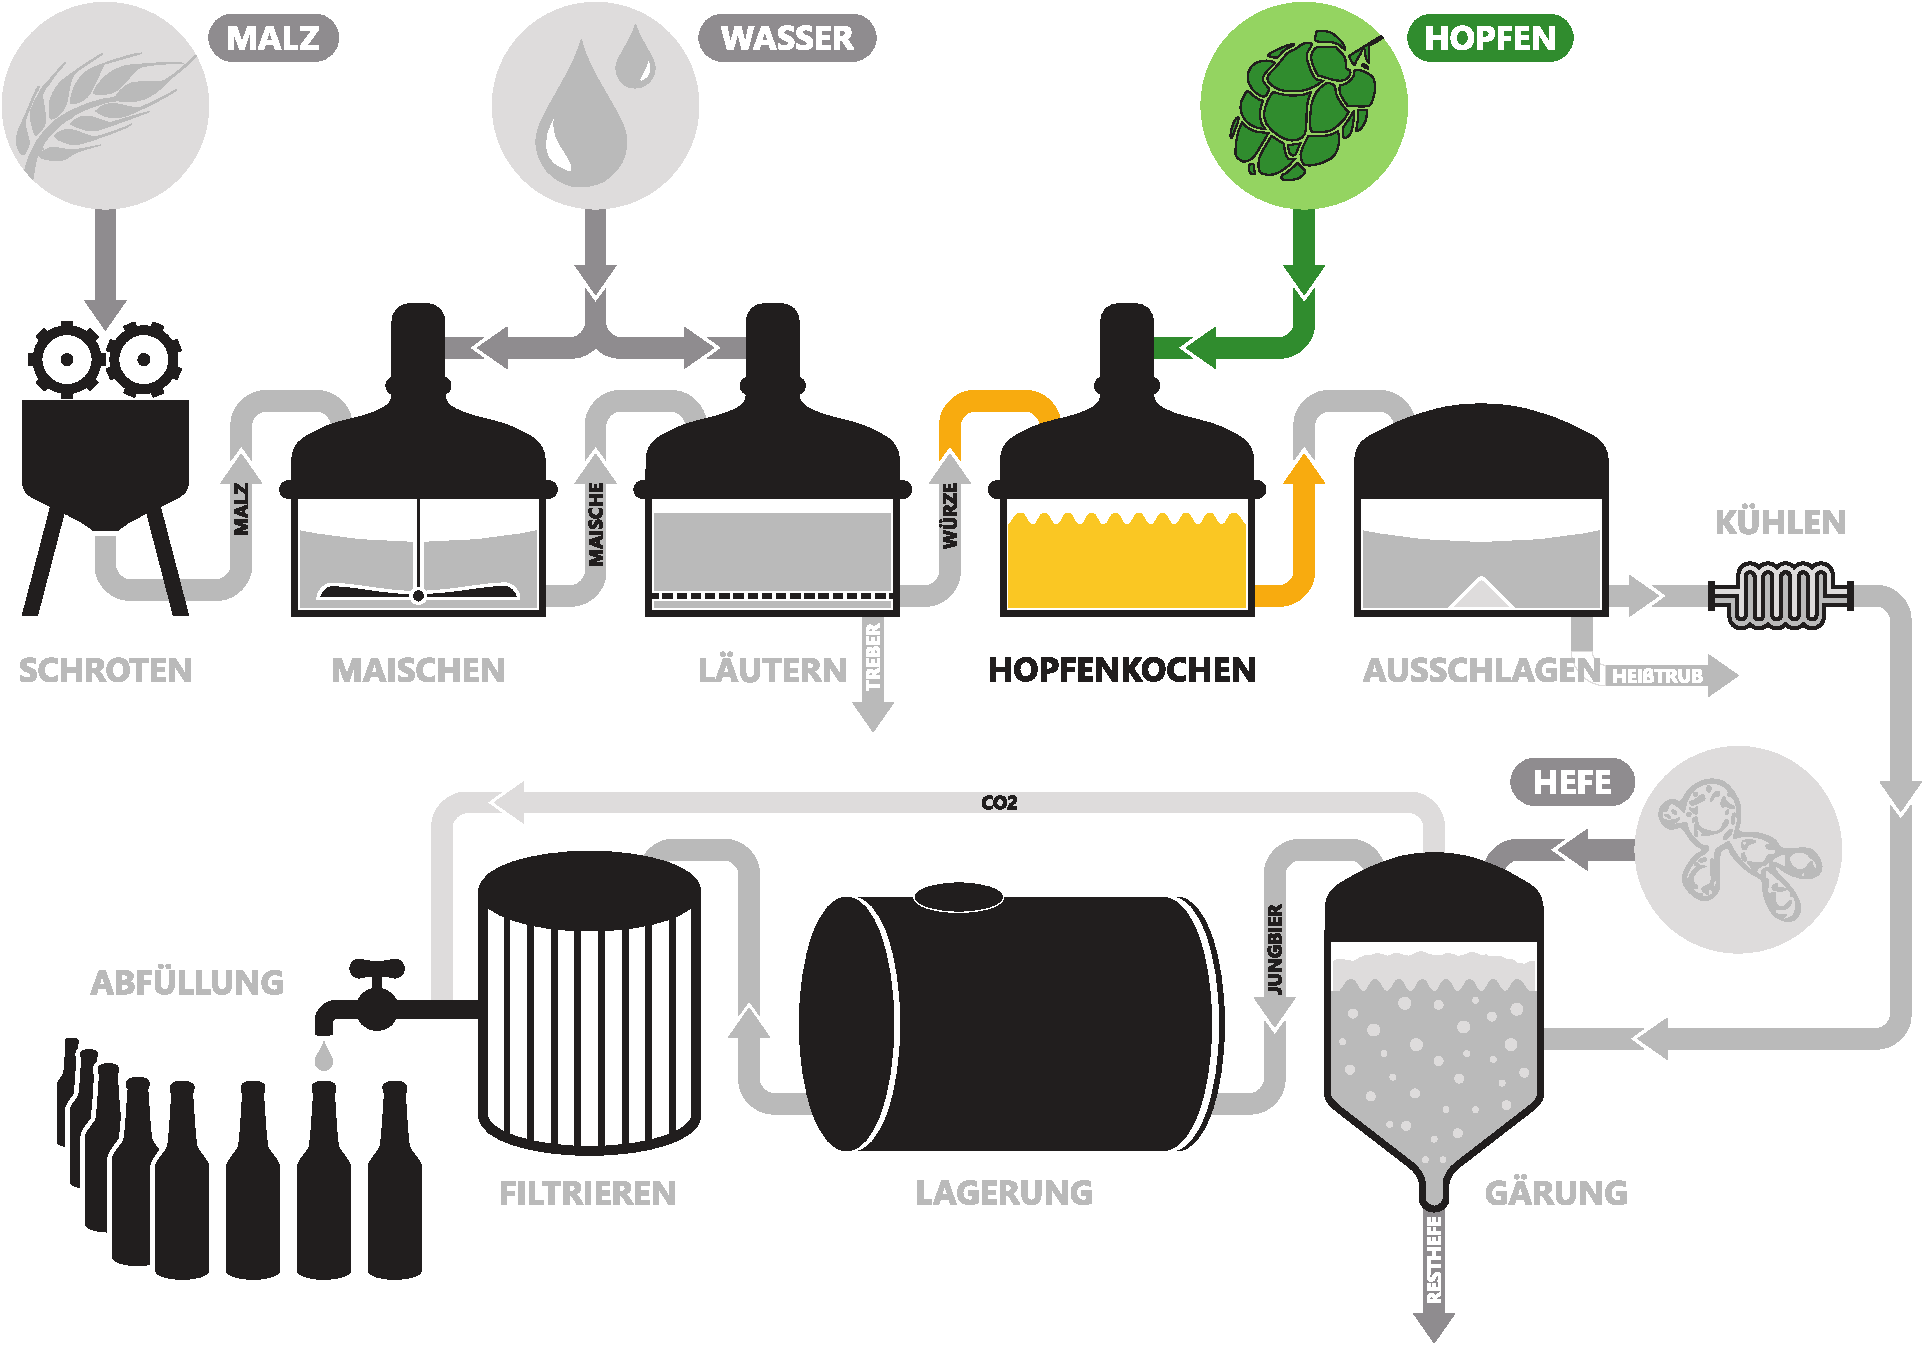
\includegraphics[width=\textwidth]{pdfs/prozess-hopfenkochen.pdf}
  \end{center}
\end{frame}
\begin{frame}{Hopfenkochen}
  \begin{block}{Zweck}
    \vspace{0.5em}

    Das Kochen hilft bei der Einstellung der endgültigen Würzekonzentration
    durch Verdunstung, zerstört Enzyme und Mikroorganismen, lässt unerwünschte
    Eiweiße gerinnen und löst Bitterstoffe des Hopfens in der Würze.

  \end{block}

  \begin{block}{Ablauf}
    \begin{enumerate}
      \item Erhitzen bis die Würze kocht
      \item Zugabe des \emph{Bitterhopfens}
      \item Zugabe des \emph{Aromahopfens} zum Ende
    \end{enumerate}
  \end{block}
\end{frame}
\begin{frame}{Hopfenseihen und Ausschlagen}
  \begin{center}
    \vspace{0.5cm}
    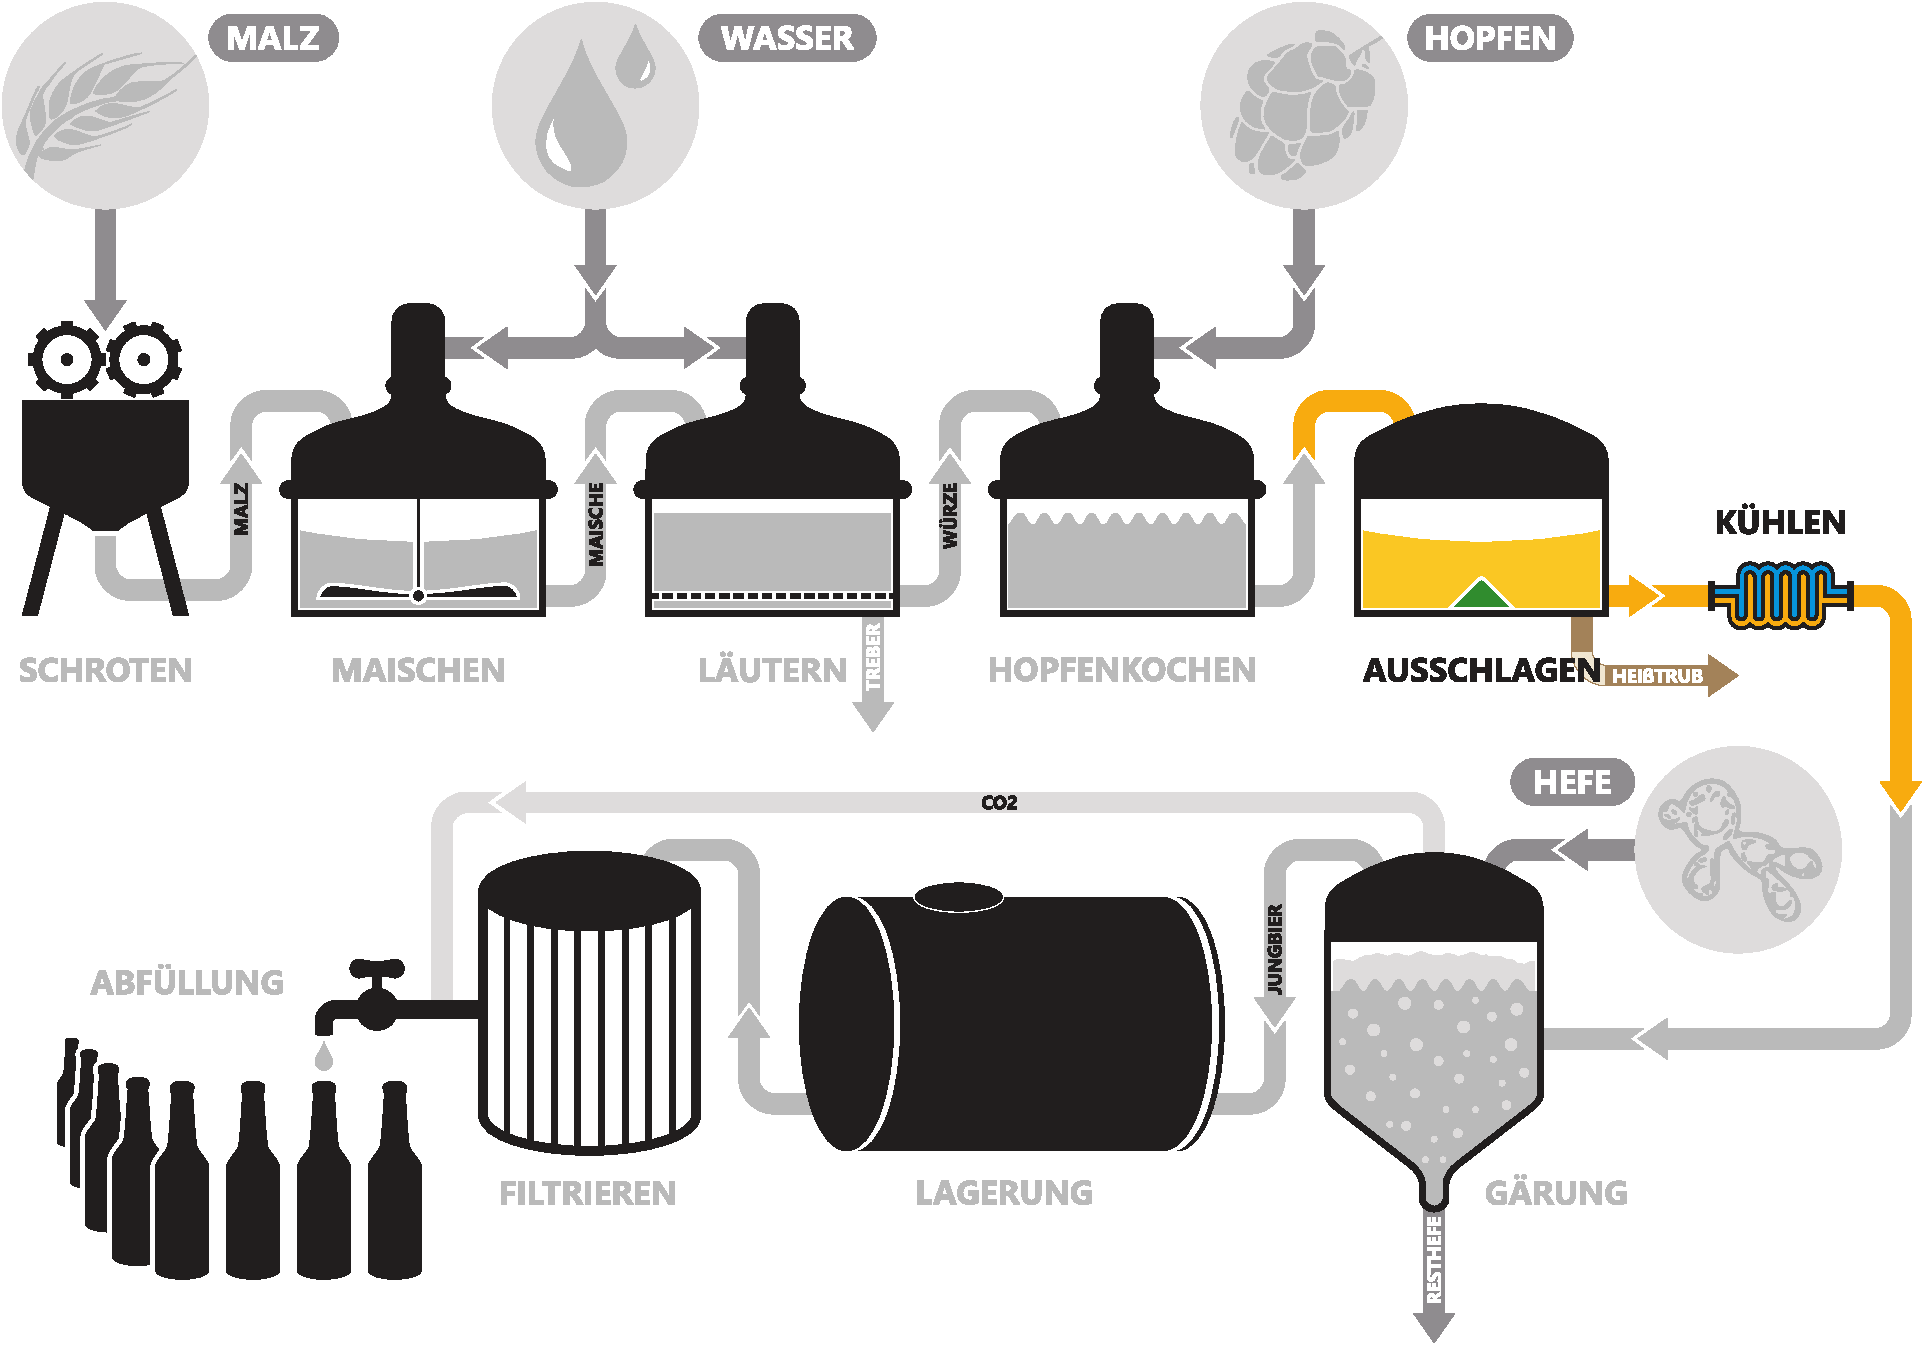
\includegraphics[width=\textwidth]{pdfs/prozess-ausschlagen.pdf}
  \end{center}
\end{frame}
\begin{frame}{Hopfenseihen und Ausschlagen}
  \begin{block}{Zweck}
    \vspace{0.5em}

    Trennung der Würze vom Hopfen, geronnenen Eiweißen und anderen
    Reststoffen. Verschiedene Methoden führen zum Ziel, allerdings ist die
    Erzeugung eines \emph{Trubkegels} durch einen \emph{Whirlpool} einfach und
    effizient. Eine schnelle Abkühlung ist erforderlich um die
    \emph{Nachisomesierung} zu reduzieren und schnell mit der \forward{Gärung}
    zu beginnen.

  \end{block}

  \begin{block}{Ablauf}
    \begin{enumerate}
      \item Würze abkühlen lassen bis die Flüssigkeit ruht
      \item Rühren der noch heißen Würze bis ein Strudel entsteht
      \item Pausieren bis der Strudel sich beruhigt hat
      \item Ablaufenlassen der Würze und dabei eventuell Nachfiltern
    \end{enumerate}
  \end{block}
\end{frame}
\begin{frame}{Gärung}
  \begin{center}
    \vspace{0.5cm}
    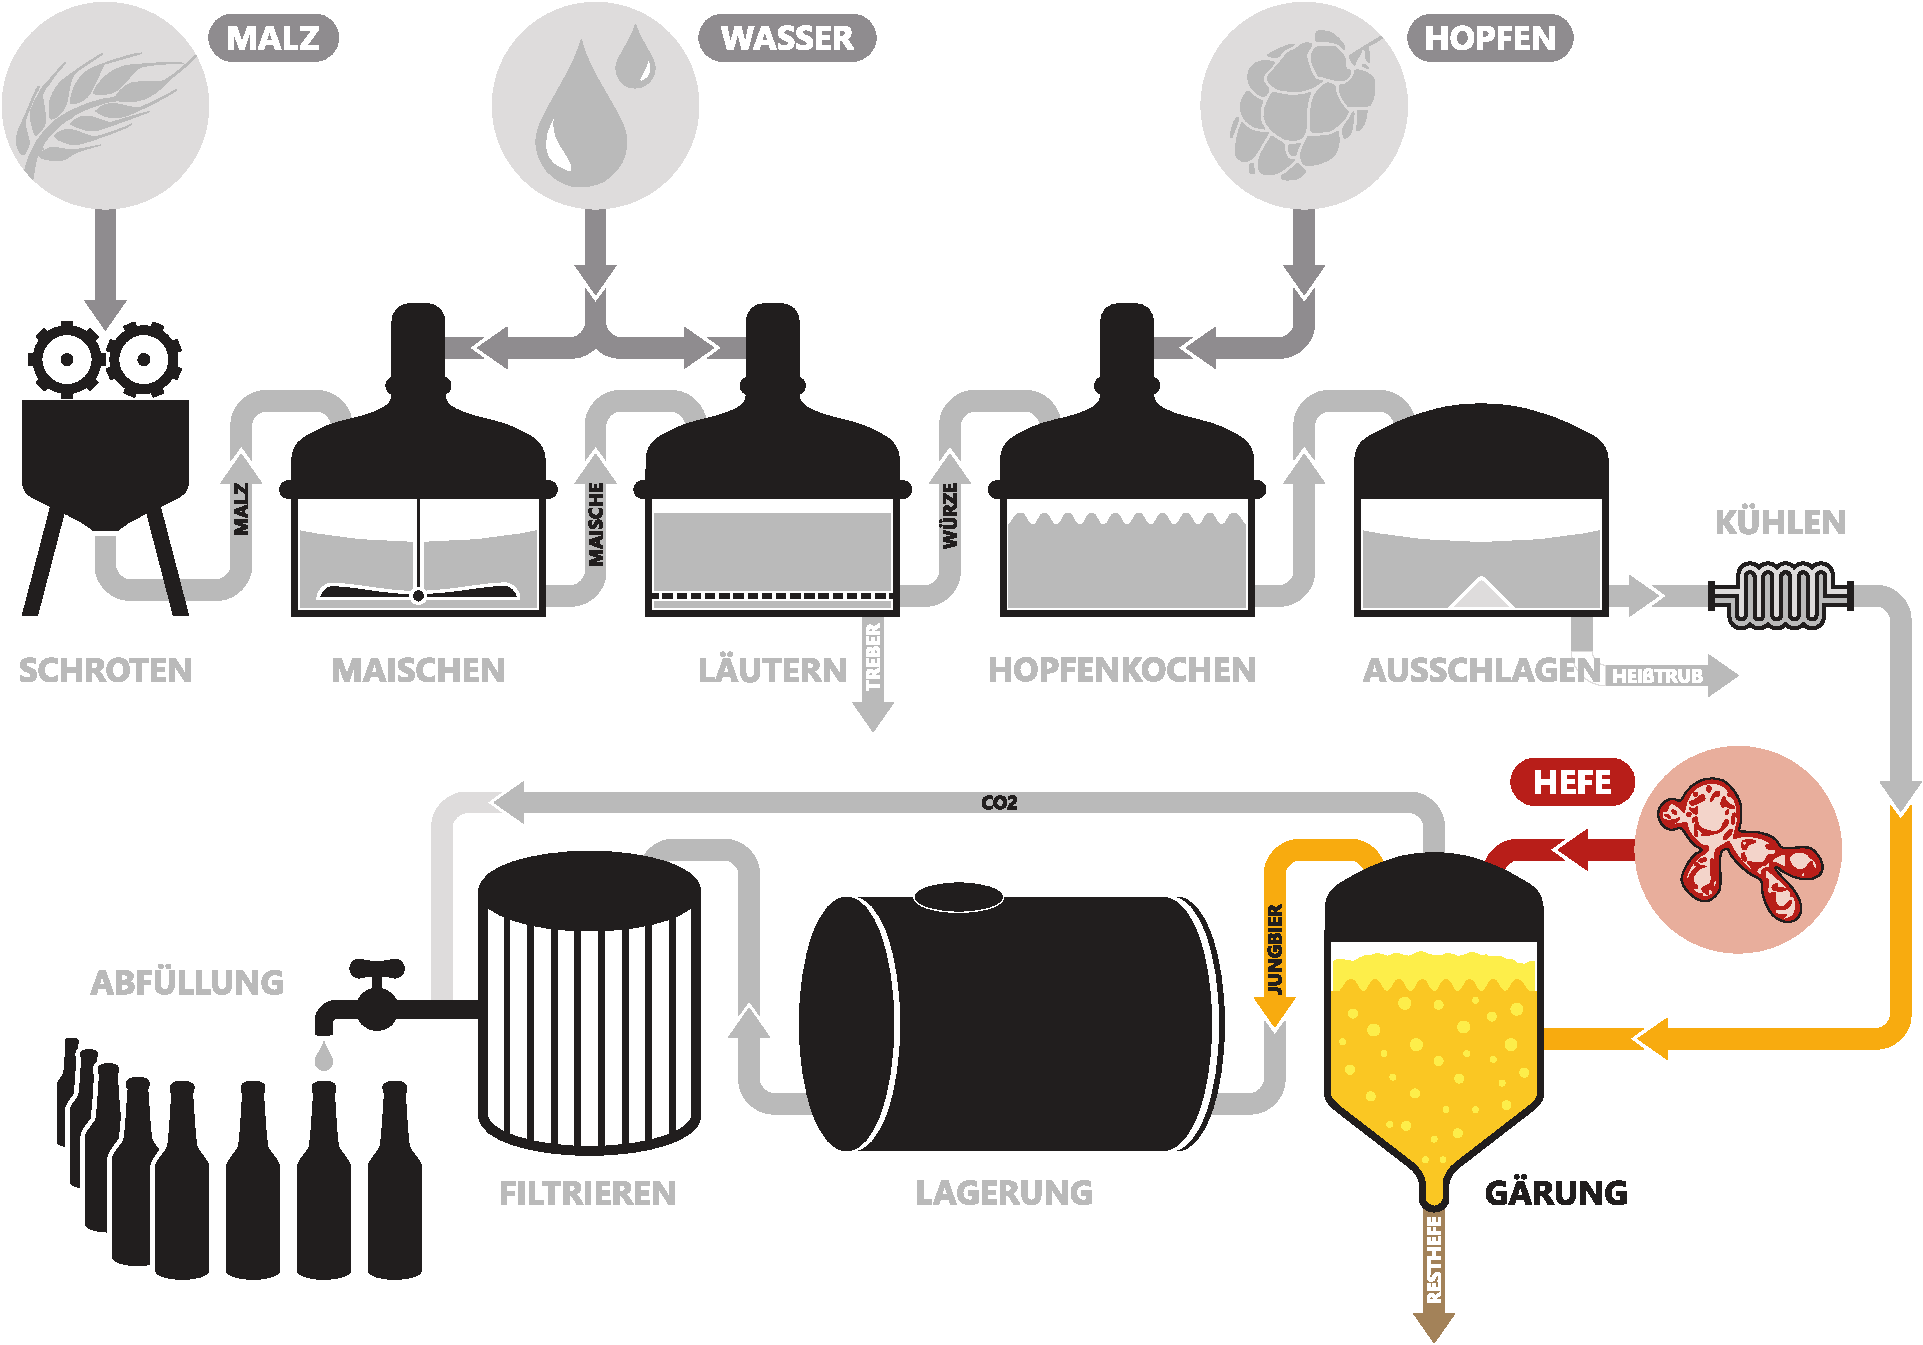
\includegraphics[width=\textwidth]{pdfs/prozess-gaerung.pdf}
  \end{center}
\end{frame}
\begin{frame}{Gärung}
  \begin{block}{Zweck}
    \vspace{0.5em}

    Umwandlung der löslichen Zucker durch Hefe in Alkohol und \ce{CO2}. Bei der
    \emph{Flaschengärung} entfallen die weitere \forward{Lagerung} und das
    endgültige \forward{Abfüllen}, da hier das \ce{CO2} und die Hefe in der
    Flasche verbleiben.

  \end{block}

  \begin{block}{Ablauf}
    \begin{enumerate}
      \item Zieltemperatur in Abhängigkeit der Hefe einstellen
      \item Gegebenenfalls die Hefe \enquote{starten}
      \item Hefe der Würze zugeben und warten \dots
    \end{enumerate}
  \end{block}
\end{frame}
\begin{frame}{Lagerung und Abfüllung}
  \begin{center}
    \vspace{0.5cm}
    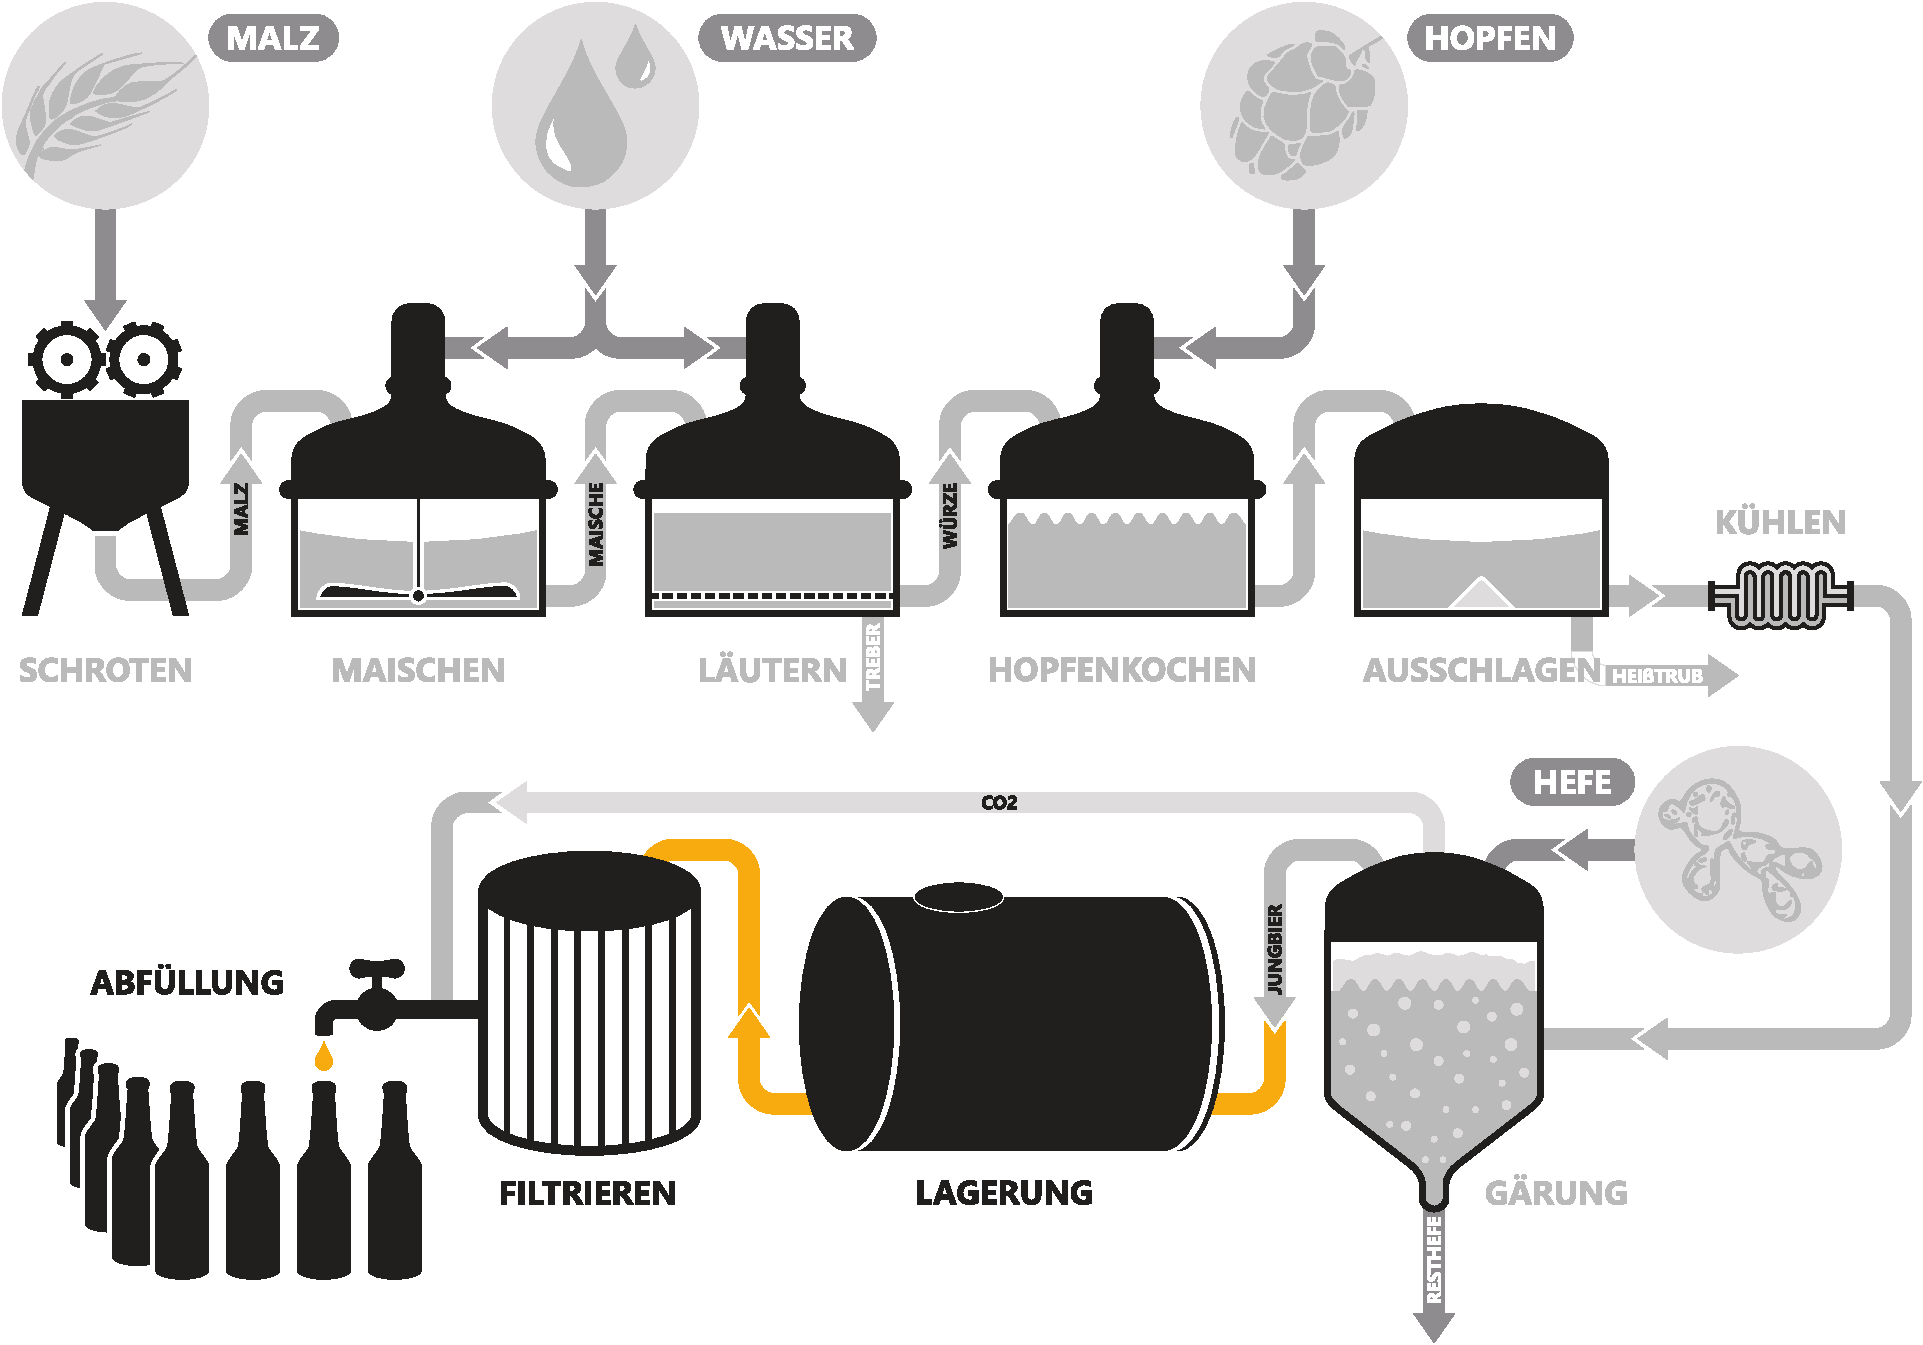
\includegraphics[width=\textwidth]{pdfs/prozess-ende.pdf}
  \end{center}
\end{frame}
\begin{frame}{Lagerung und Abfüllung}
  \begin{block}{Zweck}
    \vspace{0.5em}

    Endgültige Reifung des \emph{Jungbieres} zur Bindung des \ce{CO2}s und
    Entwicklung des geschmacklichen Endziels. Dies kann zwei Wochen bis zwei
    Monate dauern. Letztmalige Filtration ermöglicht eine kommerziell erwünschte
    Klarheit bevor das Bier abschließend abgefüllt wird.

  \end{block}

  \begin{block}{Ablauf}
    \begin{enumerate}
      \item \emph{Schlauchung} des Biers in Lagertanks
      \item Filtrieren
      \item Abfüllung in Dosen, Flaschen und Fässer
    \end{enumerate}
  \end{block}
\end{frame}

\section{Tipps}

\begin{frame}{Vermeidung von Infektionen}

  Während des Brau- und Gärprozesses ist die Würze bzw. das Bier der Umgebung
  ausgesetzt. Um Geschmacksbeeinträchtigungen vorzubeugen, sollte der Kontakt
  mit Sauerstoff soweit wie möglich reduziert und \emph{nach} dem Hopfenkochen
  alles was mit der Würze in Berührung kommt abgekocht oder anderweitig
  sterilisiert werden.

\end{frame}
\begin{frame}{Einflüsse auf die Schaumhaltbarkeit}
  \begin{block}{Malz}
    \vspace{0.5em}
    Optimaler Eiweißlösungsgrad von \SIrange{39}{42}{\percent}
  \end{block}
  \begin{block}{Maische}
    \vspace{0.5em}
    Verhinderung des Lipidabbaus beim Einmaischen durch Eimaischtemperatur >
    \SI{60}{\percent}, Auslassen der Eiweißrast und kürzeren Maischzeiten
  \end{block}
  \begin{block}{Würze}
    \vspace{0.5em}
    Einbringen eines hohen Gehaltes an α-Säure, schonende und kurze
    Kochzeit sowie Verwendung gerbstofffreier Hopfenextrakte
  \end{block}
  \begin{block}{Gärung}
    \vspace{0.5em}
    Verringerung der Kontaktzeit zwischen Hefe und Jungbier durch kurze,
    kräftige und kalte Gärung
  \end{block}
\end{frame}
\begin{frame}{Minimalausstattung}
  \begin{itemize}
    \item Koch- und Gärgefäß, Läuterbottich mit Läuterblech
    \item Messbecher, grobe und feine Waagen
    \item Großer, stabiler Kochlöffel
    \item Thermometer bis \SI{100}{\celsius} und Bierwürzespindel
    \item Bügelflaschen
  \end{itemize}
\end{frame}
\begin{frame}{Nützliche Links}
  \begin{table}
    \arrayrulecolor{white}
    \begin{tabular}{ll}
      \textbf{Shops}
        & \href{http://www.hobbybrauerversand.de}{hobbybrauerversand.de}\\
        & \href{http://www.braupartner.de}{braupartner.de}\\
        & \href{http://www.hopfen-der-welt.de}{hopfen-der-welt.de}\\
        \midrule
      \textbf{Anleitungen}
        & \href{http://brauanleitung.de}{brauanleitung.de}\\
        & \href{http://www.besser-bier-brauen.de}{besser-bier-brauen.de}\\
        & \href{http://hobbybrauer.de/forum/wiki}{hobbybrauer.de Wiki}\\
        \midrule
      \textbf{Berechnungen}
        & \href{http://fabier.de}{fabier.de}\\
        \midrule
      \textbf{Software}
        & \href{http://www.joerum.de/kleiner-brauhelfer}{joerum.de/kleiner-brauhelfer}\\
        \midrule
      \textbf{Rezepte}
        & \href{https://www.maischemalzundmehr.de}{maischemalzundmehr.de}\\
        & \href{http://meinsudhaus.de/bier-rezepte}{meinsudhaus.de/bier-rezepte}\\
        & \href{http://www.bieraromarad.de}{bieraromarad.de}\\
        \midrule
      \textbf{Fehler}
        & \href{http://hobbybrauer.de/forum/wiki/doku.php/bier:fehler}{hobbybrauer.de Wiki}
    \end{tabular}
  \end{table}
\end{frame}

\section{Heute}

\begin{frame}{American Pale Ale}
  Anders als englische IPAs dominieren bei den APAs fruchtige Zitrus- und
  Grapefruitaromen durch den wenig-bitteren \emph{Cascade}-Hopfen.

  \begin{block}{Zielwerte}
    \begin{itemize}
      \item Stammwürze \SI{13}{\dP} und Restextrakt \SI{3}{\dP}
      \item Alkohol \SI{5.4}{\volP}
      \item 27 IBU Bittere und 22 EBC Farbe
    \end{itemize}
  \end{block}
\end{frame}
\begin{frame}{Brauplan}
  \begin{columns}[T, onlytextwidth]
    \column{0.5\textwidth}
      \begin{block}{Schüttung}
        \begin{itemize}
          \item \SI{4200}{\gram} Pale Ale Malz
          \item \SI{400}{\gram} Crystal 40 oder CARAMÜNCH\textregistered\  II
        \end{itemize}
      \end{block}
      \begin{block}{Maische}
        \begin{itemize}
          \item Single-Step Infusion
          \item 60 Minuten
          \item \SI{66}{\celsius}
        \end{itemize}
      \end{block}

    \column{0.5\textwidth}
      \begin{block}{Hopfen}
        \begin{itemize}
          \item \SI{10}{\gram} Columbus, 60 Minuten
          \item \SI{20}{\gram} Cascade, 15 Minuten
          \item \SI{20}{\gram} Cascade, 5 Minuten
          \item \SI{20}{\gram} Cascade im Whirlpool
        \end{itemize}
      \end{block}
      \begin{block}{Gärung und Abfüllung}
        \begin{itemize}
          \item Wyeast 1056 American Ale
          \item Karbonisierung auf \SI{4}{\gram\per\liter} \ce{CO2}
        \end{itemize}
      \end{block}

  \end{columns}
\end{frame}

\end{document}
